\documentclass[DM,authoryear,toc]{lsstdoc}
% lsstdoc documentation: https://lsst-texmf.lsst.io/lsstdoc.html
\input{meta}

% Package imports go here.

% Local commands go here.

%If you want glossaries
%\input{aglossary.tex}
%\makeglossaries

\title{Periodicity Analysis in Alert Production}

% Optional subtitle
% \setDocSubtitle{A subtitle}

\author{%
Anastasios Tzanidakis
}

\author{%
Eric Bellm
}

\setDocRef{DMTN-221}
\setDocUpstreamLocation{\url{https://github.com/lsst-dm/dmtn-221}}

\date{\vcsDate}

% Optional: name of the document's curator
% \setDocCurator{The Curator of this Document}

\setDocAbstract{%
The baselined timeseries features to be computed in Alert Production include a Lomb-Scargle periodogram.  We assess the computational and scientific performance of several configurations on simulated alert data.
}


% Change history defined here.
% Order: oldest first.
% Fields: VERSION, DATE, DESCRIPTION, OWNER NAME.
% See LPM-51 for version number policy.
\setDocChangeRecord{%
  \addtohist{1}{YYYY-MM-DD}{Unreleased.}{Eric Bellm}
}


\begin{document}

% Create the title page.
\maketitle
% Frequently for a technote we do not want a title page  uncomment this to remove the title page and changelog.
% use \mkshorttitle to remove the extra pages

% ADD CONTENT HERE
% You can also use the \input command to include several content files.


\begin{figure*}
  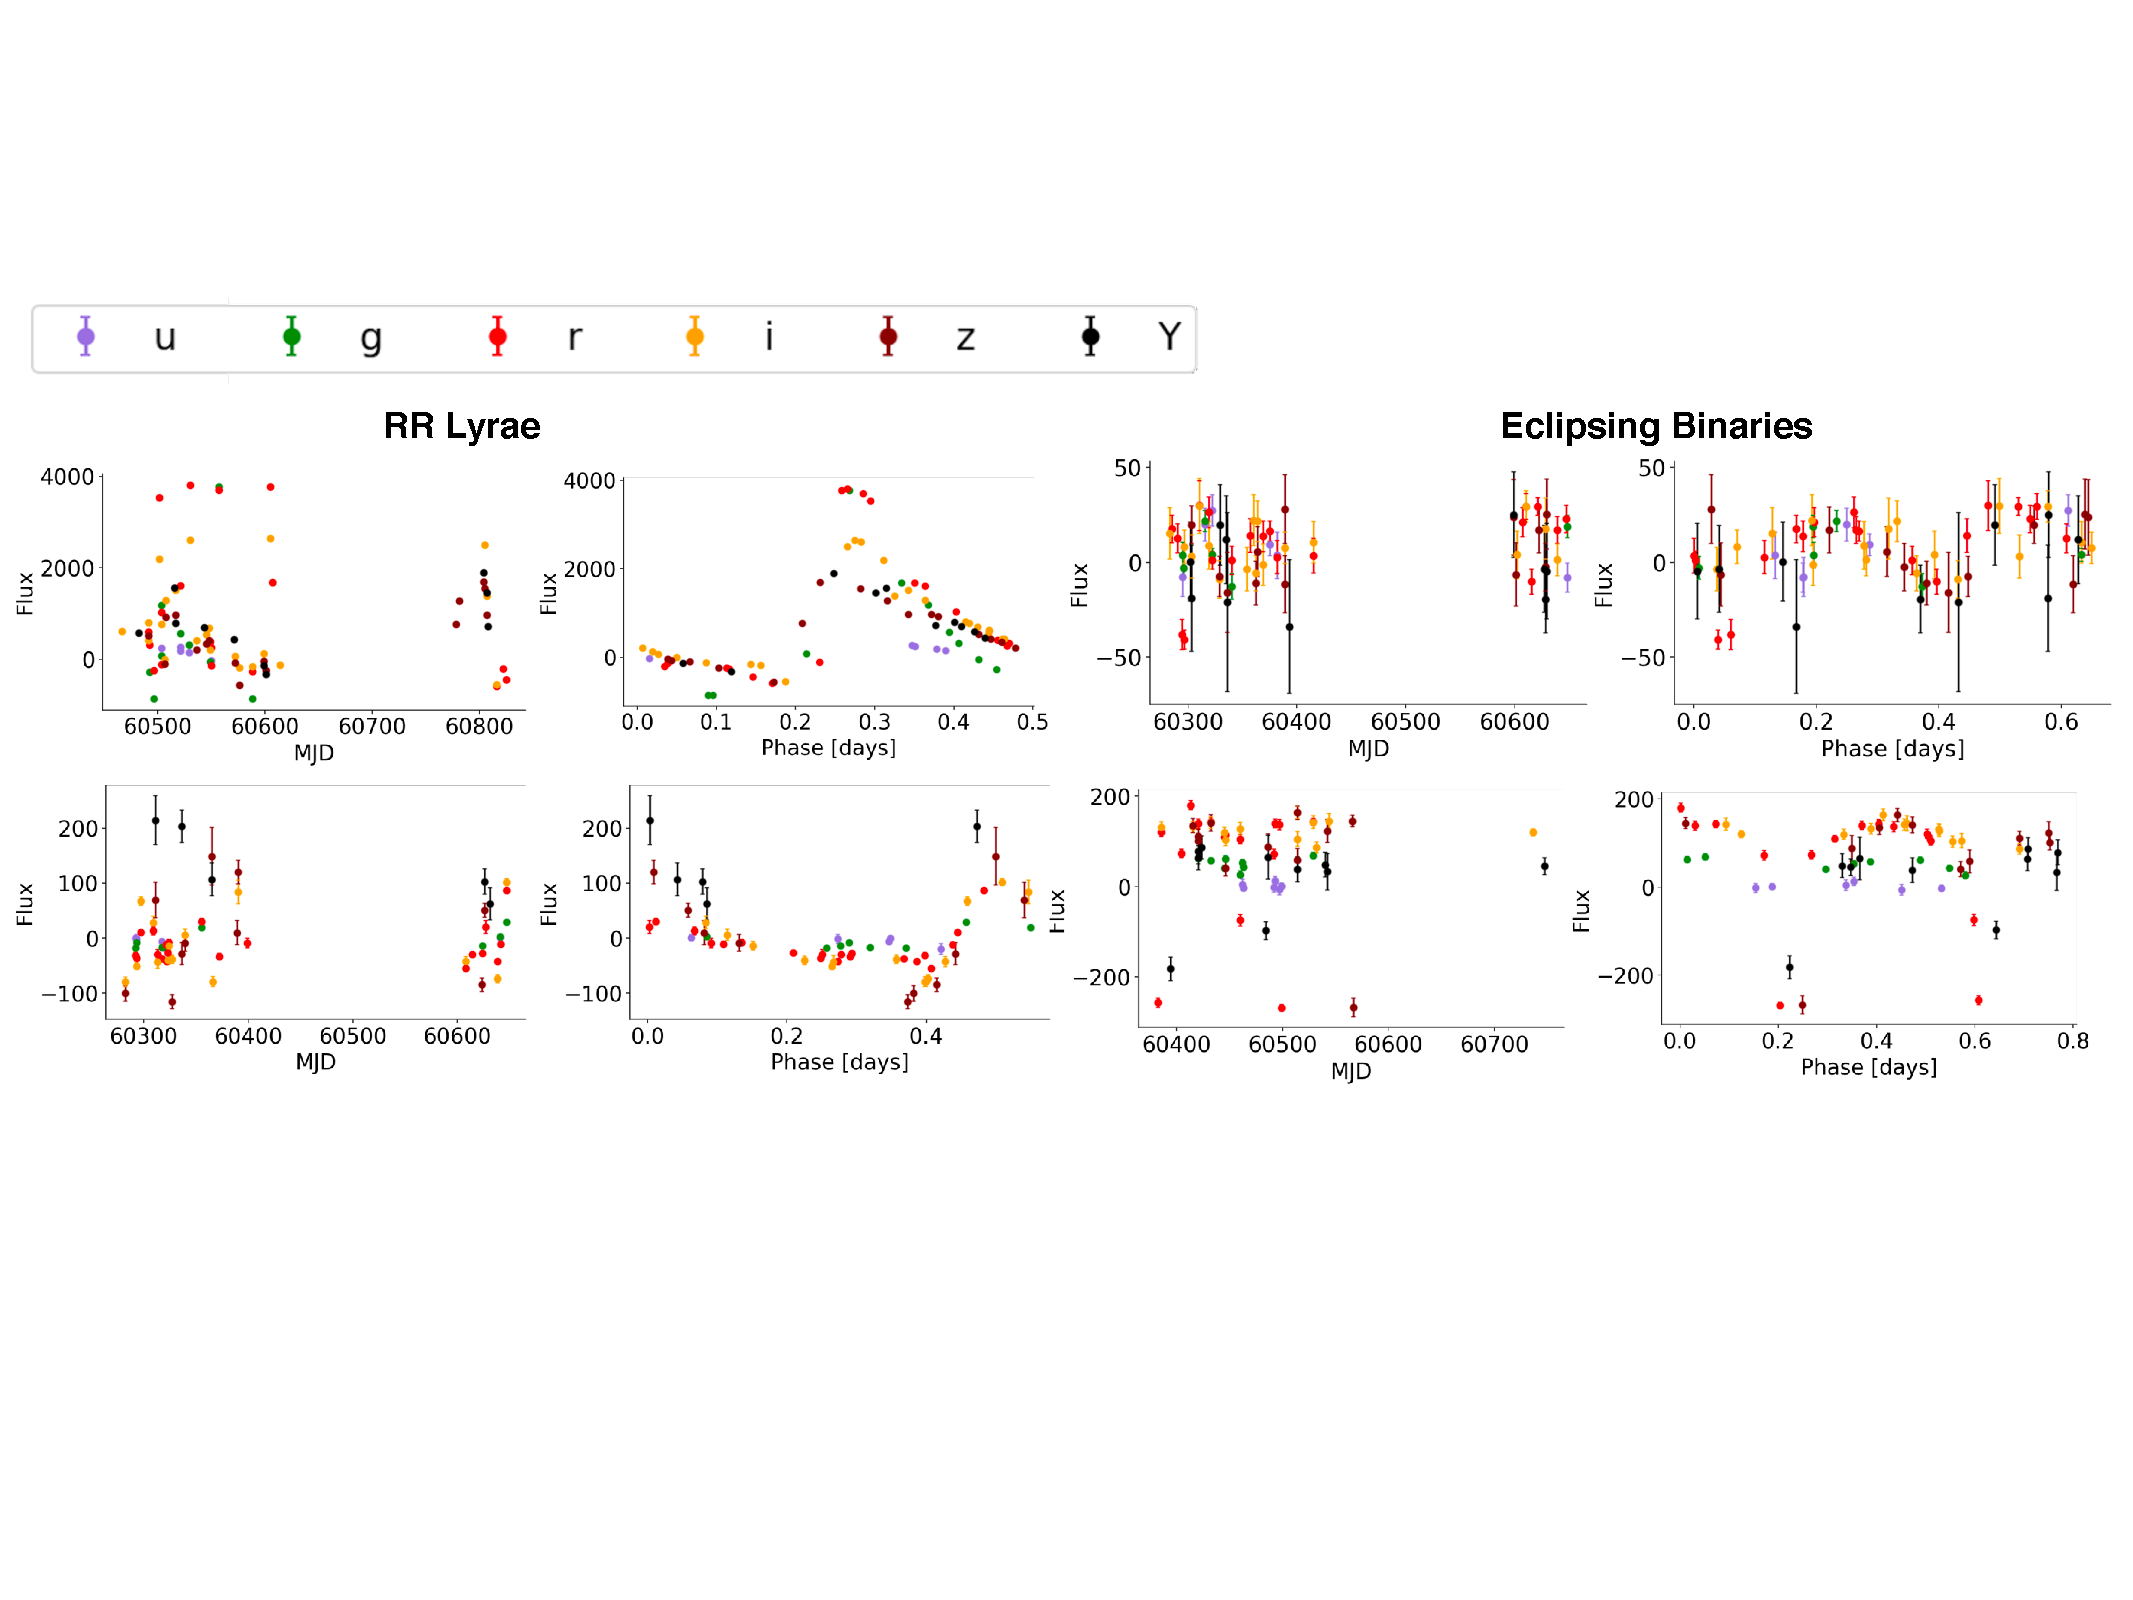
\includegraphics[width=0.8\textwidth]{figures/lightcurve_demo.pdf}
  \centering 
  \caption{The above panels demonstrate the multi-band light curves simulated from ElasTiCC using RR Lyrae (left panel) and Eclipsing Binaries (right panel). The first column of each panel shows the observed light curves, and the second the phase folded light curves at the correct period after 12 months.}
  \label{fig:comp}
\end{figure*}



\appendix
% Include all the relevant bib files.
% https://lsst-texmf.lsst.io/lsstdoc.html#bibliographies
\section{References} \label{sec:bib}
\renewcommand{\refname}{} % Suppress default Bibliography section
\bibliography{local,lsst,lsst-dm,refs_ads,refs,books}

% Make sure lsst-texmf/bin/generateAcronyms.py is in your path
\section{Acronyms} \label{sec:acronyms}
\addtocounter{table}{-1}
\begin{longtable}{p{0.145\textwidth}p{0.8\textwidth}}\hline
\textbf{Acronym} & \textbf{Description}  \\\hline

AGN & active galactic nuclei \\\hline
CCD & Charge-Coupled Device \\\hline
DC2 & Data Challenge 2 (DESC) \\\hline
DIA & Difference Image Analysis \\\hline
DM & Data Management \\\hline
DMTN & DM Technical Note \\\hline
EB & ExaByte \\\hline
HR & Human Resources \\\hline
LSST & Legacy Survey of Space and Time (formerly Large Synoptic Survey Telescope) \\\hline
SDSS & Sloan Digital Sky Survey \\\hline
\end{longtable}

% If you want glossary uncomment below -- comment out the two lines above
%\printglossaries





\end{document}
